\documentclass{beamer}

% Packages
\usepackage[english]{babel}
\usepackage[utf8]{inputenc}
\usepackage{graphicx}
\usepackage{tabularx}

% Theme
\usetheme{Antibes}
\useoutertheme{umbcfootline}
\setfootline{\insertshortinstitute, \insertshortdate \hfill Slide \insertframenumber/\inserttotalframenumber}

% Title
\title{Oasis: Part of the GIRAF System}
\author{Henrik Klarup, Jens Mohr Mortensen, and Dan Stenholt M\o{}ller}
\institute[AAU]{Aalborg University}
\date{Juni 26, 2012}

\begin{document}

\begin{frame}
	\titlepage
\end{frame}

\begin{frame}
	\frametitle{Agenda}
	\begin{itemize}
		\item Multiprojekt Beskrivelse
		\item GIRAF Arkitekturen
		\item Udviklingsmetode
		\item Oasis
		\item Testing
		\item Reflektion
		\item Konklusion
		\item Demonstration
	\end{itemize}
\end{frame}

\section{Multiprojekt Beskrivelse}

\begin{frame}
	\frametitle{Multiprojekt Beskrivelse}
	\begin{itemize}
		\item Flere grupper
		\item Videreudvikling af tidligere projekt (GIRAF)
		\item Hj\ae{}lpev\ae{}rkt\o{}jer til b\o{}rn med ASD og deres p\ae{}dagoer
	\end{itemize}
	\begin{quote}
		\textit{``How can we ease the daily life for children with ASD and their guardians, while complying with the study regulation?''}
	\end{quote}
\end{frame}

\section{GIRAF Arkitekturen}

\begin{frame}
	\frametitle{GIRAF Arkitekturen}
	\begin{itemize}
		\item Android
	\end{itemize}
	\begin{figure}[!h]
		\centering
			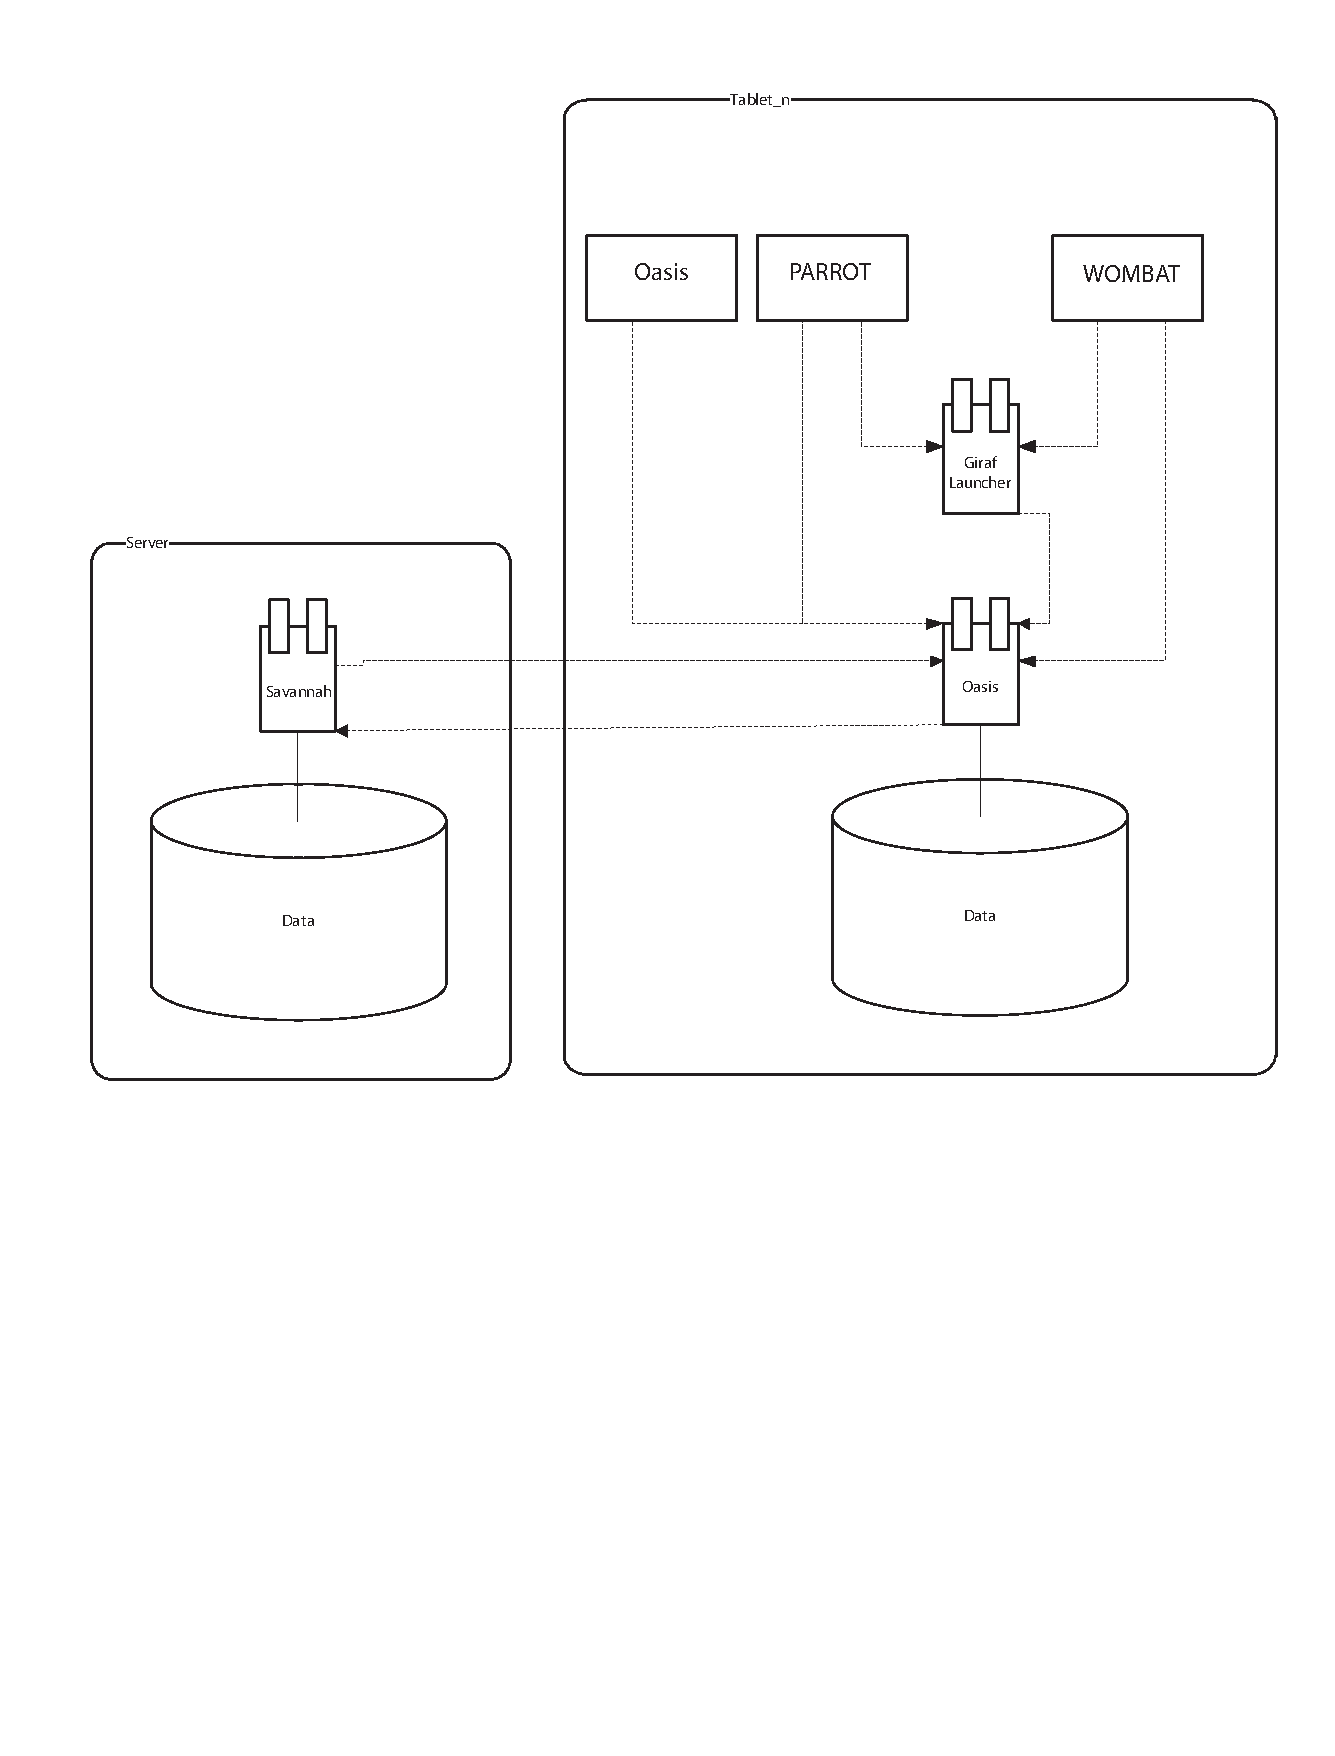
\includegraphics[width=0.8\textwidth]{../../../Reports/Group_4/Tex/Images/Giraf_comp.pdf}
		\label{fig:Giraf_comp}
	\end{figure}
\end{frame}

\section{Udviklingsmetode}

\subsection{Hvorfor Agilt?}

\begin{frame}
	\frametitle{Hvorfor Agilt?}
	
	\begin{figure}[!h]
		\centering
			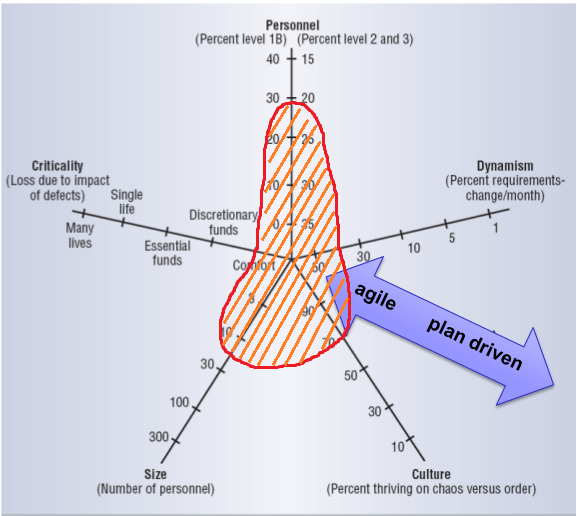
\includegraphics[width=0.7\textwidth]{PolarChart.PNG}
		\label{fig:Polar Chart}
	\end{figure}
\end{frame}

\subsection{Scrum of Scrums}

\begin{frame}
	\frametitle{Scrum of Scrums}
	
	\begin{itemize}
		\item Godt til et multiprojekt
		\item Hvert team er selvorganiseret
		\item Scrum Modifikationer:
			\begin{itemize}
				\item Kortere sprint l\ae{}ngde
				\item Ingen Scrum Master eller Product Owner
				\item Scrum of Scrums m\o{}de 
			\end{itemize}
	\end{itemize}
\end{frame}

\section{Oasis}

\begin{frame}
	\frametitle{Oasis}
	\begin{itemize}
		\item Problem Definition
		\item Krav
		\item Valg af Database Model
		\item Systemet
		\item Local Db
		\item Library
		\item App
	\end{itemize}
\end{frame}

\subsection{Problem Definition}

\begin{frame}
	\frametitle{Problem Definition}
	
	\begin{quote}
	\textit{``How can we provide a set of tools, which can help develop applications for the GIRAF system?''}
	\end{quote}
\end{frame}

\subsection{Krav}

\begin{frame}
	\frametitle{Krav}
	
	\begin{itemize}
		\item H\aa{}ndtering af:
		\begin{itemize}
			\item Adgang
			\item Profiler
			\item Afdelinger
			\item Medier
			\item Tags
			\item Apps
		\end{itemize}
	\end{itemize}
\end{frame}

\subsection{Valg af Database Model}

\begin{frame}
	\frametitle{Valg af Database Model}
	\begin{figure}[!h]
		\centering
			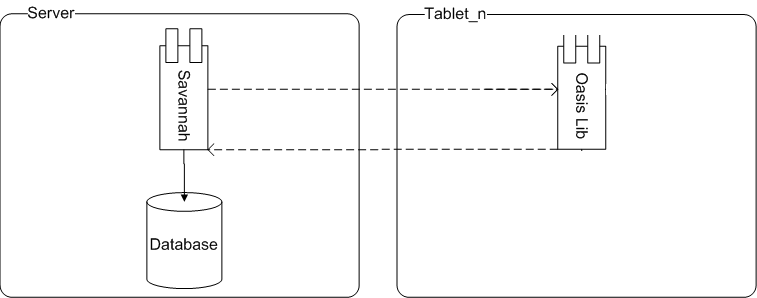
\includegraphics[width=0.7\textwidth]{kunekstern}
		\label{fig:DatabaseModel1}
	\end{figure}
	\begin{figure}[!h]
		\centering
			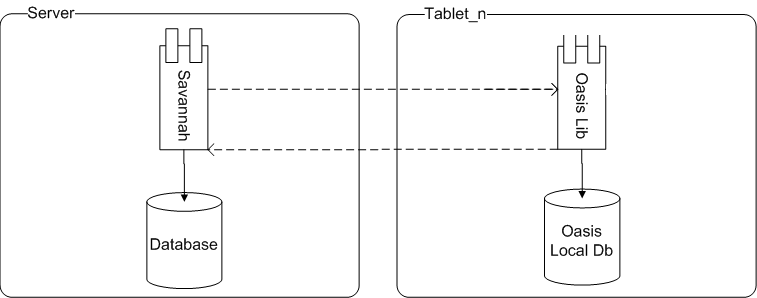
\includegraphics[width=0.7\textwidth]{localogekstern}
		\label{fig:DatabaseModel2}
	\end{figure}
\end{frame}

\subsection{Local Db}

\begin{frame}
	\frametitle{Profiler}
	
	\begin{figure}[!h]
		\centering
			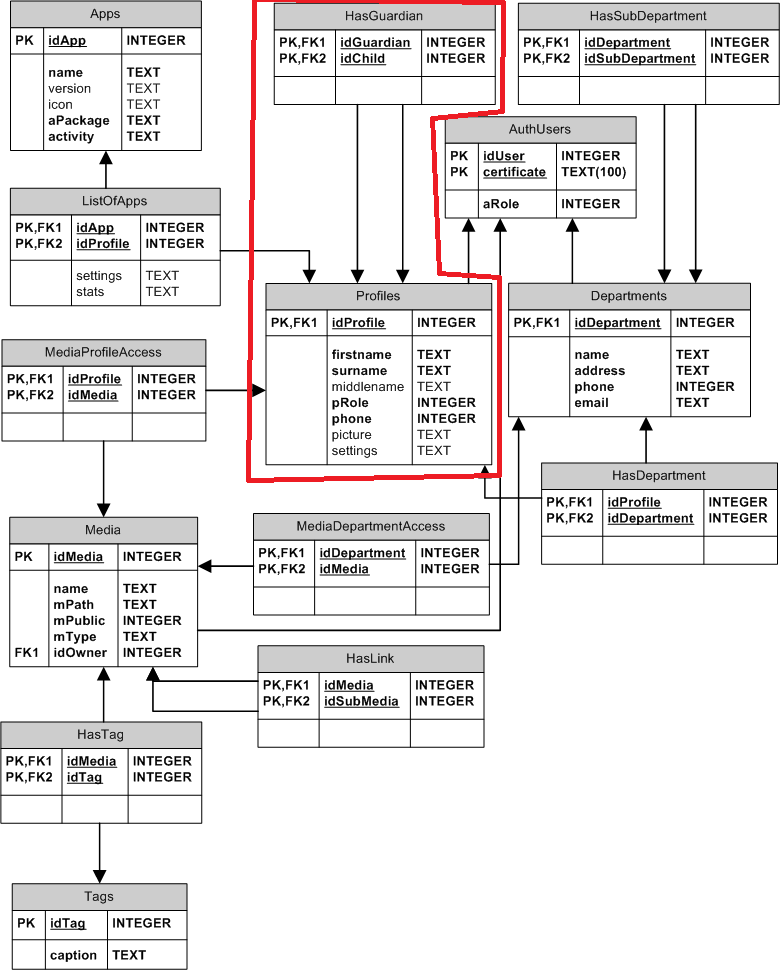
\includegraphics[width=0.5\textwidth]{dbProfiler}
		\label{fig:profiler}
	\end{figure}
\end{frame}

\begin{frame}
	\frametitle{Afdelinger}
	
	\begin{figure}[!h]
		\centering
			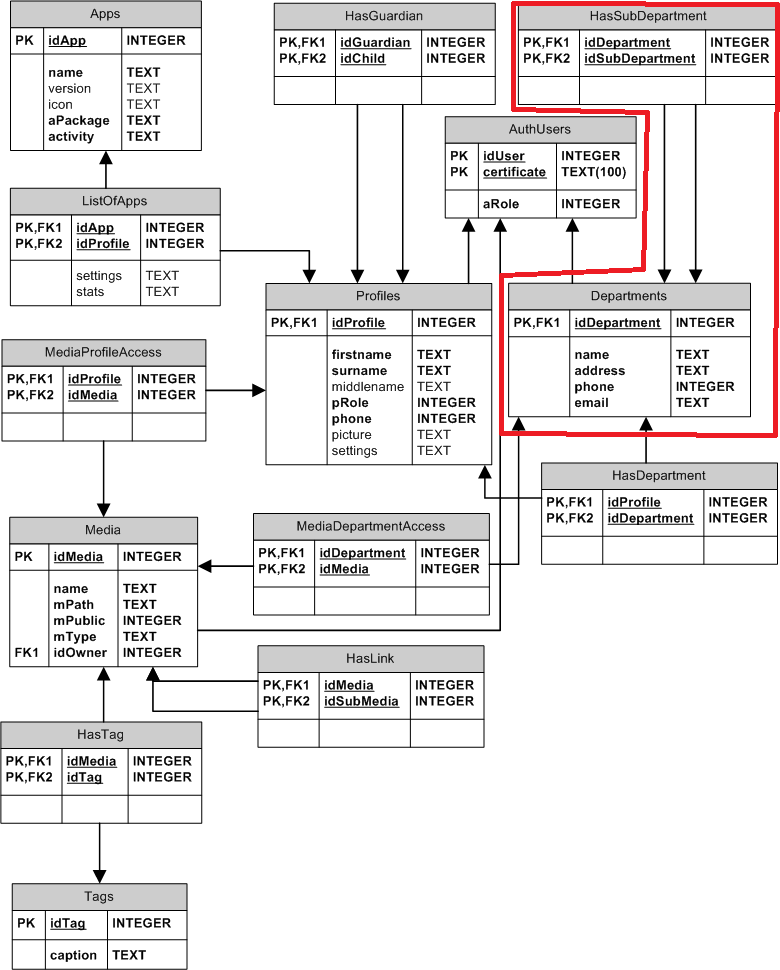
\includegraphics[width=0.5\textwidth]{dbAfdelinger}
		\label{fig:Afdelinger}
	\end{figure}
\end{frame}

\begin{frame}
	\frametitle{Profiler/Afdelinger}
	
	\begin{figure}[!h]
		\centering
			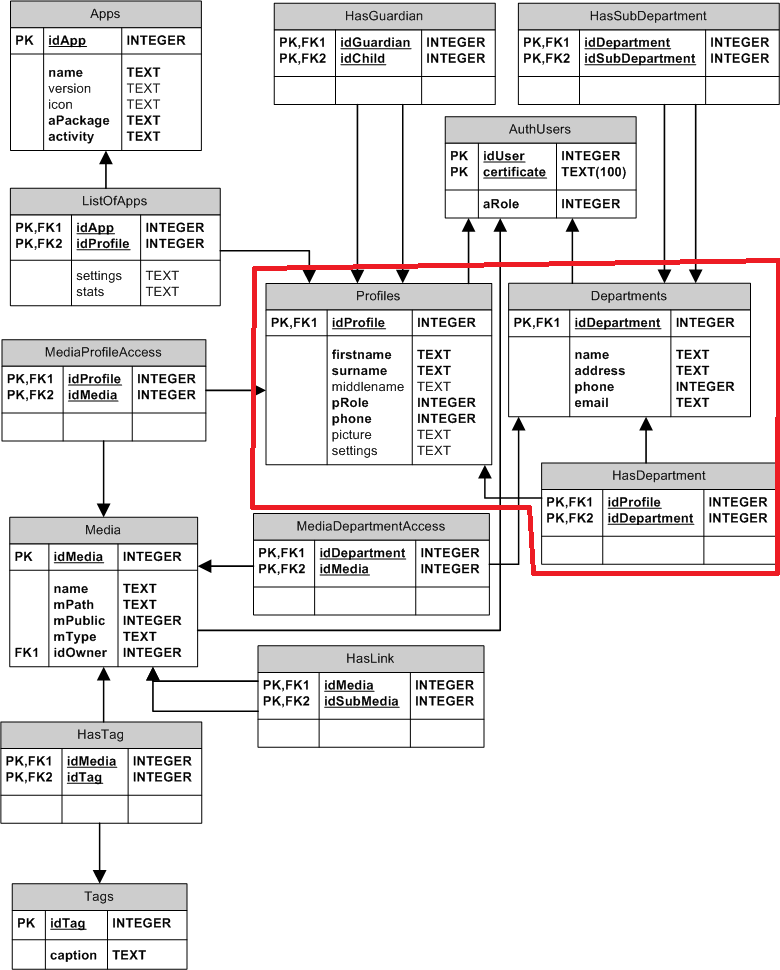
\includegraphics[width=0.5\textwidth]{dbProfil-Afdeling}
		\label{fig:ProfilerAfdelinger}
	\end{figure}
\end{frame}

\begin{frame}
	\frametitle{Certifikater}
	
	\begin{figure}[!h]
		\centering
			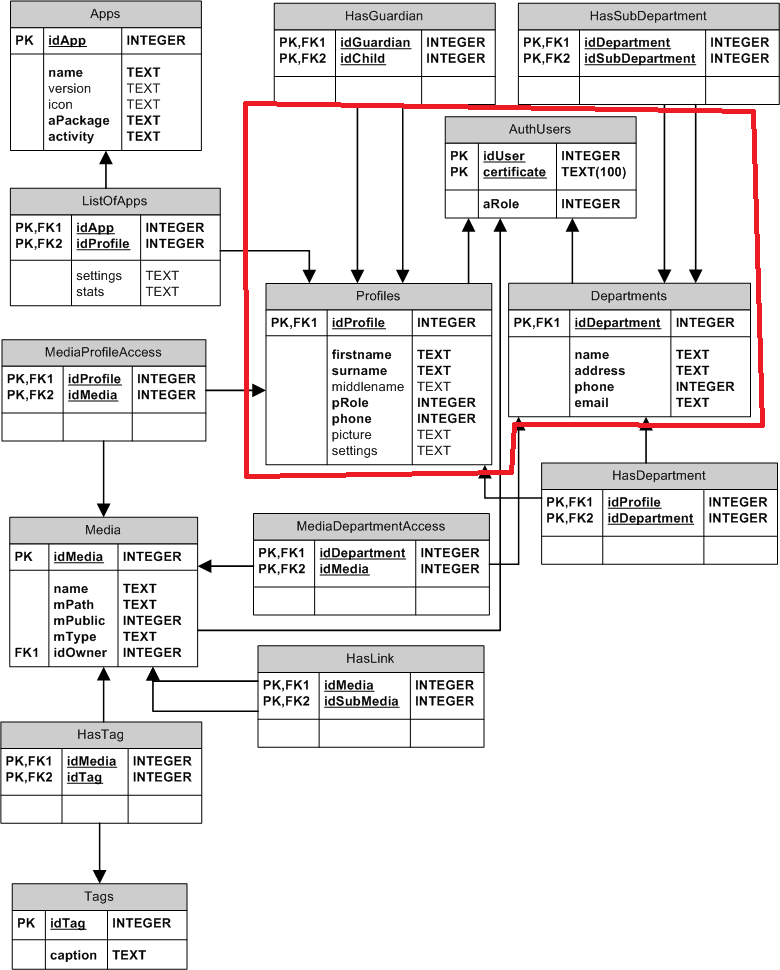
\includegraphics[width=0.5\textwidth]{dbCertificate}
		\label{fig:Certifikater}
	\end{figure}
\end{frame}

\begin{frame}
	\frametitle{Applikationer}
	
	\begin{figure}[!h]
		\centering
			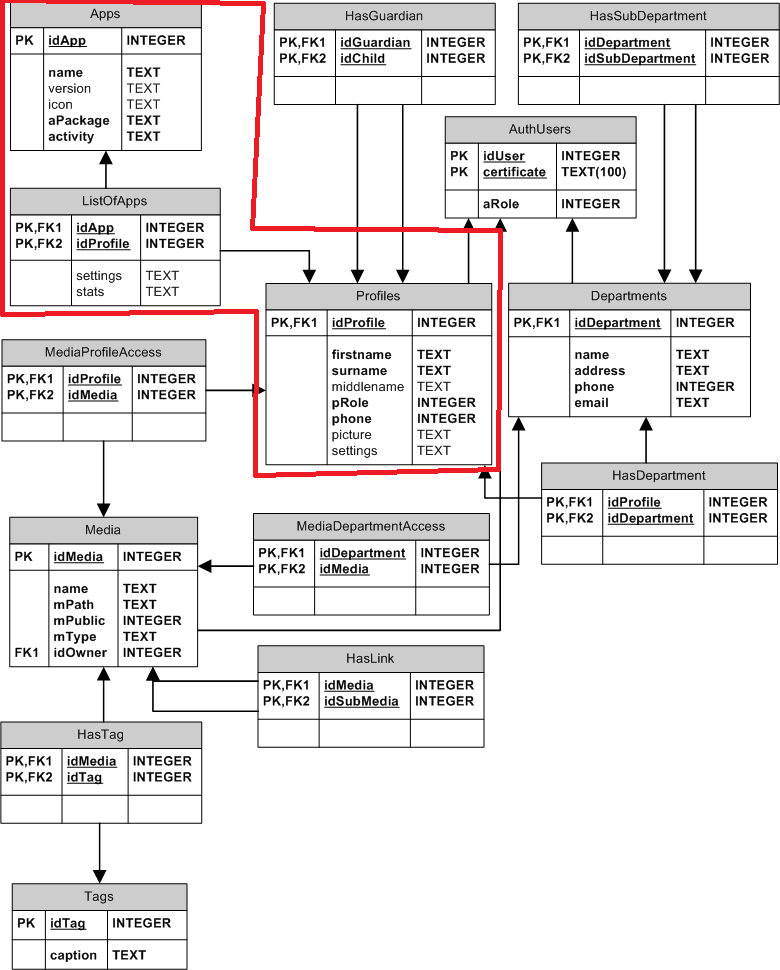
\includegraphics[width=0.5\textwidth]{dbApps}
		\label{fig:Applikationer}
	\end{figure}
\end{frame}

\begin{frame}
	\frametitle{Medier}
	
	\begin{figure}[!h]
		\centering
			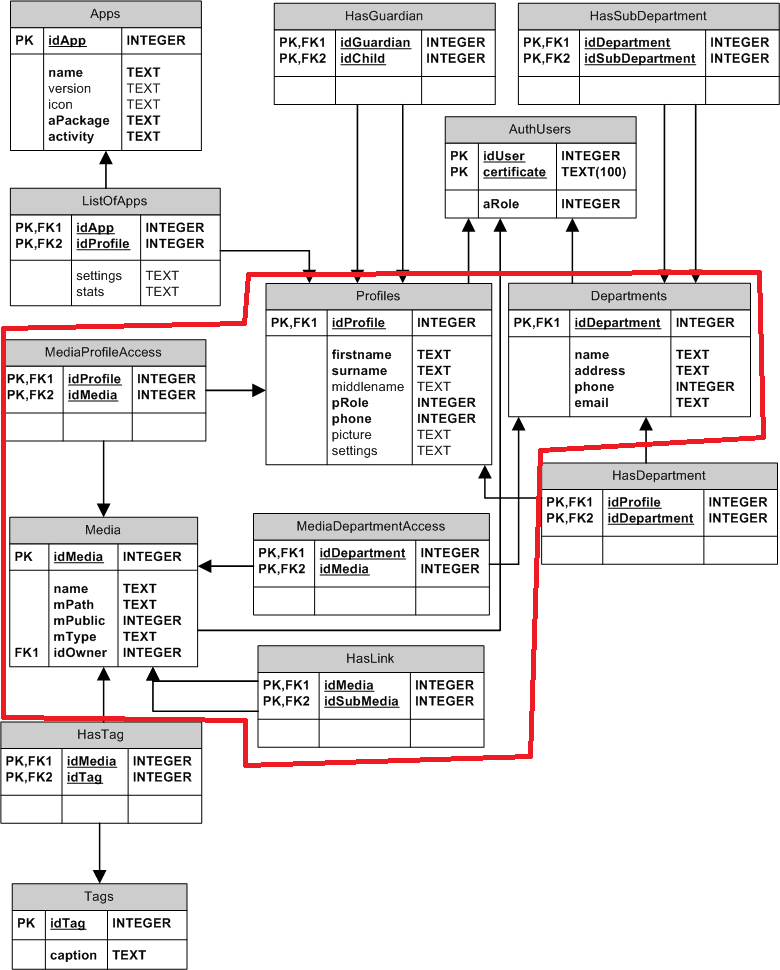
\includegraphics[width=0.5\textwidth]{dbMedia}
		\label{fig:Medier}
	\end{figure}
\end{frame}

\begin{frame}
	\frametitle{Tags}
	
	\begin{figure}[!h]
		\centering
			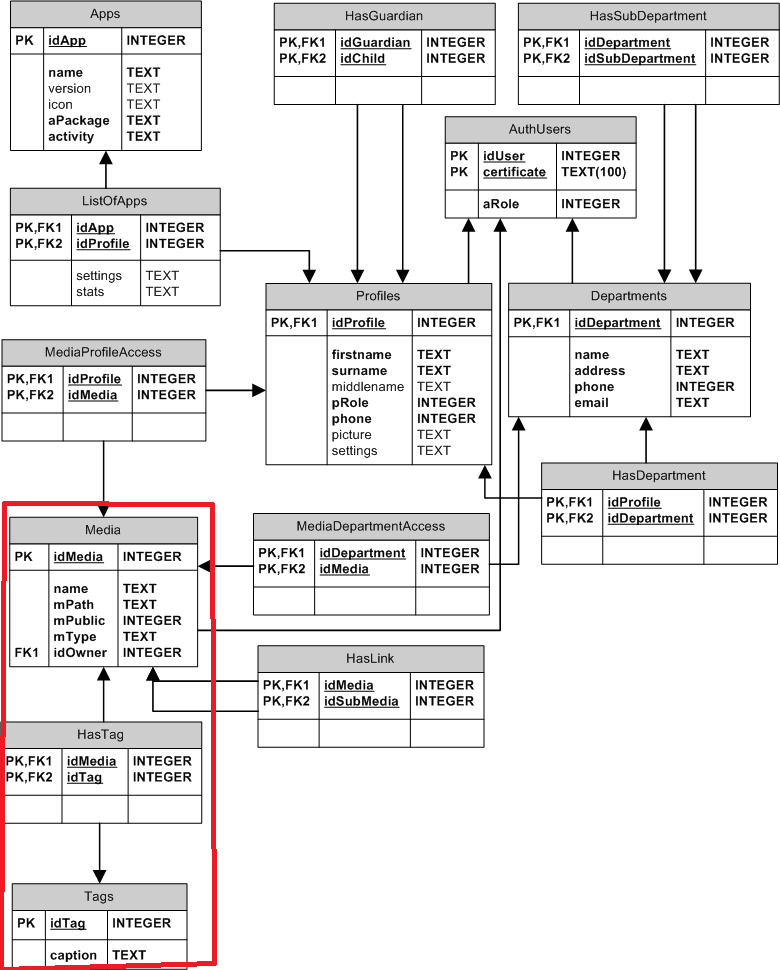
\includegraphics[width=0.5\textwidth]{dbTags}
		\label{fig:Tags}
	\end{figure}
\end{frame}



\begin{frame}
	\frametitle{Anvendelse}
	
	\begin{itemize}
		\item Vedligeholder r\ae{}kker i tabellerne
		\begin{itemize}
			\item Opret
			\item L\ae{}s
			\item Modificer
			\item Slet
		\end{itemize}
	\end{itemize}
\end{frame}

\subsection{Library}

\begin{frame}
	\frametitle{Library}
	\begin{itemize}
		\item Bindeled mellem apps og databasen
		\item Sikrer overholdelse af adgangskrav
		\item Tilbyder Db funktioner tilpasset apps
	\end{itemize}
	\begin{itemize}
		\item Synkroniser med Savannah
		\begin{itemize}
			\item Ikke implementeret
		\end{itemize}
	\end{itemize}
\end{frame}

\subsection{App}

\begin{frame}
	\frametitle{App}
	\begin{itemize}
		\item Demo app
		\item Anvender Library'et
		\item Giver administrations muligheder
	\end{itemize}
\end{frame}

\section{Testing}

\begin{frame}
	\frametitle{Testing}
	\begin{itemize}
		\item Unit test
		\item Usability test
	\end{itemize}
\end{frame}

\subsection{Unit Test}

\begin{frame}
	\frametitle{Unit Test}
	\begin{itemize}
		\item Dynamic white box tests
		\item Test-to-pass/test-to-fail
		\item Test af library og database
		\item 88 ud af 89 bestod
	\end{itemize}
\end{frame}

\subsection{Usability Test}

\begin{frame}
	\frametitle{Usability Test}
	\begin{itemize}
		\item Test af app'en
		\item Ekspert test
		\item IDA test
	\end{itemize}
	\begin{table}[!h]
	\centering
		\begin{tabular}{| p{2cm} | m{7cm} |}
			\hline
			\textbf{Issues} 	& \textbf{Description} \\ \hline
			
			\textbf{Cosmetic:}	& Profile id was showing. \\ 
								& ``Add child'' not clear how to. \\ \hline
							
			\textbf{Serious:}	& Too many options, missing the overview. \\
								& Difficult finding a child profile. \\ \hline
						
			\textbf{Critical:} 	& Data availability unclear. \\ \hline
		\end{tabular}
	\label{tab:usability_test_results}
\end{table}
\end{frame}

\section{Reflektion}

\begin{frame}
	\frametitle{Reflektion}
	\begin{itemize}
		\item Scrum erfaringer
		\begin{itemize}
			\item Sv\ae{}rt at isolere sig
			\begin{itemize}
				\item Tilf\o{}jelser til sprint backlog'en
				\item Unit test blev nedprioriteret i forhold til nye opgaver
			\end{itemize}
		\end{itemize}
		\item Test erfaringer
		\begin{itemize}
			\item Unit test skulle ikke nedprioriteres
			\item Integrations test blev udf\o{}rt l\o{}bende
		\end{itemize}
		
	\end{itemize}
\end{frame}

\section{Konklusion}

\begin{frame}
	\frametitle{Konklusion}
	\begin{itemize}
		\item Multiprojekt Beskrivelse
		\item GIRAF Arkitekturen
		\item Udviklingsmetode
		\item Oasis
		\item Testing
		\item Reflektion
	\end{itemize}
\end{frame}

\section{Demonstration}

\begin{frame}
	\frametitle{Demonstration}
	\begin{itemize}
		\item \textbf{LIVE} demonstration af Oasis App'en
	\end{itemize}
\end{frame}

\end{document}